% Rebuild from figures/: pdflatex -interaction=nonstopmode -halt-on-error protocol.tex
\documentclass[border=2pt]{standalone}
\usepackage[T1]{fontenc}
\usepackage{helvet}
\renewcommand{\familydefault}{\sfdefault}
\usepackage{amsmath}
\usepackage{anyfontsize}
\usepackage{tikz}
\usetikzlibrary{arrows.meta,calc}
\definecolor{ink}{HTML}{28333F}
\definecolor{muted}{HTML}{596673}
\definecolor{rule}{HTML}{D7DDE2}
\definecolor{blue}{HTML}{2A78D6}
\definecolor{orange}{HTML}{C65B29}
\definecolor{green}{HTML}{287C68}
\begin{document}
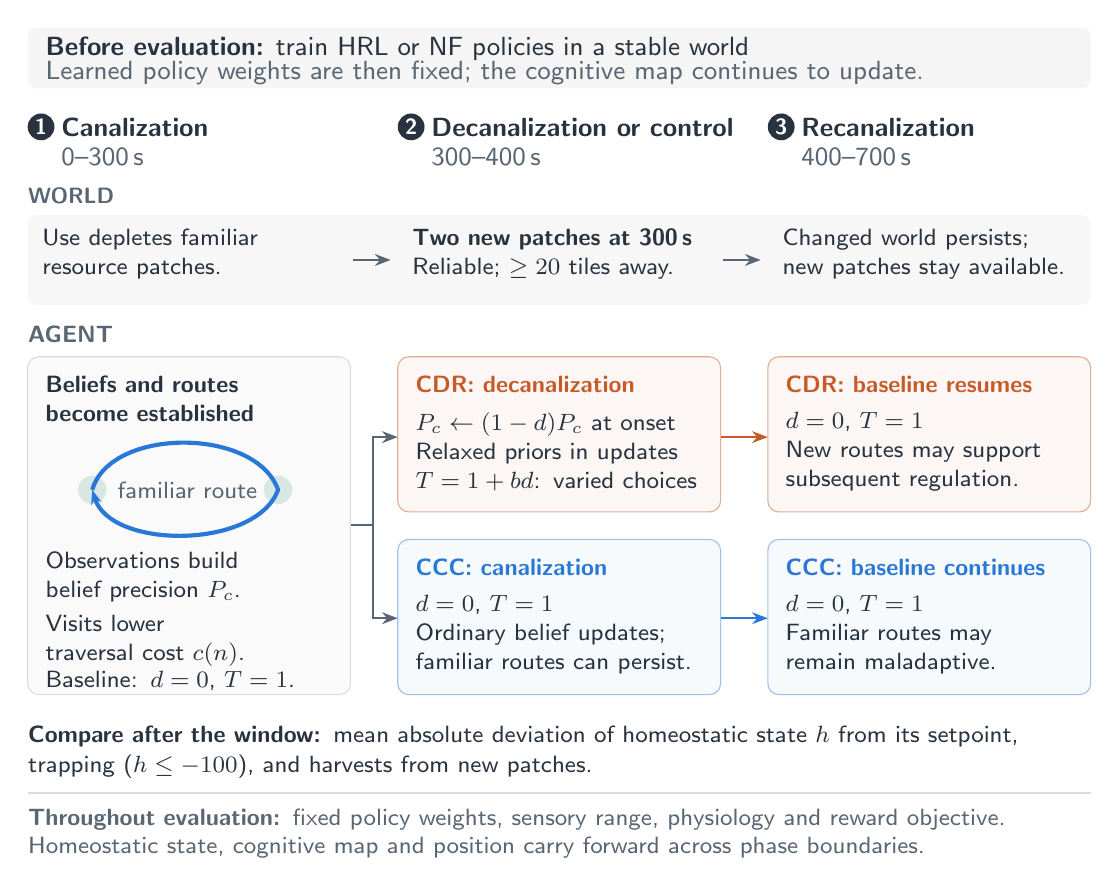
\begin{tikzpicture}[x=1cm,y=1cm,
  every node/.style={font=\fontsize{9}{11}\selectfont,text=ink,inner sep=0pt},
  flow/.style={-{Stealth[length=2mm]},line width=0.8pt,draw=muted},
  copy/.style={align=left,anchor=north west,text width=3.68cm,font=\fontsize{8.5}{10.5}\selectfont},
  smallcopy/.style={align=left,anchor=north west,text width=3.68cm,font=\fontsize{8}{10}\selectfont}]
\path[use as bounding box] (0,0) rectangle (13.5,10.6);

% Training precedes the three-phase evaluation; the two objectives use the same protocol.
\fill[black!4,rounded corners=3pt] (0,9.83) rectangle (13.5,10.6);
\node[anchor=west,font=\fontsize{9.5}{12}\selectfont] at (0.22,10.33)
  {\textbf{Before evaluation:} train HRL or NF policies in a stable world};
\node[anchor=west,text=muted] at (0.22,10.02)
  {Learned policy weights are then fixed; the cognitive map continues to update.};

% Equal-width phase columns are schematic, not proportional to duration.
\foreach \x/\n/\title/\timing in {
  0/1/Canalization/{0--300\,s},
  4.7/2/Decanalization or control/{300--400\,s},
  9.4/3/Recanalization/{400--700\,s}} {
  \fill[ink] (\x+0.17,9.34) circle (0.17);
  \node[text=white,font=\bfseries\fontsize{8}{9}\selectfont] at (\x+0.17,9.34) {\n};
  \node[anchor=west,font=\bfseries\fontsize{9}{11}\selectfont] at (\x+0.42,9.34) {\title};
  \node[anchor=west,text=muted] at (\x+0.42,8.96) {\timing};
}

% World changes are shared by both conditions, and persist after the window.
\node[anchor=west,font=\bfseries\fontsize{8}{10}\selectfont,text=muted] at (0,8.47) {WORLD};
\fill[black!3,rounded corners=3pt] (0,7.08) rectangle (13.5,8.22);
\node[copy] at (0.18,8.05) {Use depletes familiar\\resource patches.};
\node[copy] at (4.88,8.05) {\textbf{Two new patches at 300\,s}\\Reliable; $\geq20$ tiles away.};
\node[copy] at (9.58,8.05) {Changed world persists;\\new patches stay available.};
\draw[flow] (4.13,7.65) -- (4.61,7.65);
\draw[flow] (8.83,7.65) -- (9.31,7.65);
\node[anchor=west,font=\bfseries\fontsize{8}{10}\selectfont,text=muted] at (0,6.71) {AGENT};

% Shared experience before the intervention/control split.
\filldraw[fill=black!2,draw=rule,rounded corners=4pt] (0,2.13) rectangle (4.1,6.42);
\node[copy] at (0.22,6.18) {\textbf{Beliefs and routes\\become established}};
% A repeated circuit through familiar patches.
\fill[green!18] (0.82,4.73) circle (0.18);
\fill[green!18] (3.18,4.73) circle (0.18);
\draw[blue,line width=1.5pt,-{Stealth[length=1.8mm]}]
  (0.82,4.73) .. controls (1.05,5.53) and (2.9,5.53) .. (3.18,4.73)
  .. controls (2.9,3.97) and (1.05,3.97) .. (0.82,4.73);
\node[text=muted,font=\fontsize{8}{10}\selectfont] at (2.03,4.73) {familiar route};
\node[copy] at (0.22,3.95) {Observations build\\belief precision $P_c$.};
\node[copy] at (0.22,3.15) {Visits lower\\traversal cost $c(n)$.};
\node[copy] at (0.22,2.43) {Baseline: $d=0$, $T=1$.};

% Decanalization branch.
\filldraw[fill=orange!5,draw=orange!50,rounded corners=4pt] (4.7,4.45) rectangle (8.8,6.42);
\node[copy,text=orange] at (4.92,6.18) {\textbf{CDR: decanalization}};
\node[copy] at (4.92,5.72) {$P_c\leftarrow(1-d)P_c$ at onset\\Relaxed priors in updates\\$T=1+bd$: varied choices};
% Undisturbed branch.
\filldraw[fill=blue!4,draw=blue!45,rounded corners=4pt] (4.7,2.13) rectangle (8.8,4.1);
\node[copy,text=blue] at (4.92,3.86) {\textbf{CCC: canalization}};
\node[copy] at (4.92,3.4) {$d=0$, $T=1$\\Ordinary belief updates;\\familiar routes can persist.};

% Baseline mechanisms resume; the experience acquired is not reset.
\filldraw[fill=orange!5,draw=orange!50,rounded corners=4pt] (9.4,4.45) rectangle (13.5,6.42);
\node[copy,text=orange] at (9.62,6.18) {\textbf{CDR: baseline resumes}};
\node[copy] at (9.62,5.72) {$d=0$, $T=1$\\New routes may support\\subsequent regulation.};
\filldraw[fill=blue!4,draw=blue!45,rounded corners=4pt] (9.4,2.13) rectangle (13.5,4.1);
\node[copy,text=blue] at (9.62,3.86) {\textbf{CCC: baseline continues}};
\node[copy] at (9.62,3.4) {$d=0$, $T=1$\\Familiar routes may\\remain maladaptive.};
\draw[flow] (4.1,4.28) -- (4.39,4.28) |- (4.7,5.4);
\draw[flow] (4.39,4.28) |- (4.7,3.1);
\draw[flow,draw=orange] (8.8,5.4) -- (9.4,5.4);
\draw[flow,draw=blue] (8.8,3.1) -- (9.4,3.1);

\node[anchor=north west,align=left,text width=13.5cm,font=\fontsize{8.5}{11}\selectfont] at (0,1.74)
  {\textbf{Compare after the window:} mean absolute deviation of homeostatic state $h$ from its setpoint,\\trapping ($h\leq-100$), and harvests from new patches.};
\draw[rule] (0,0.88) -- (13.5,0.88);
\node[anchor=north west,align=left,text width=13.5cm,text=muted,font=\fontsize{8}{10}\selectfont] at (0,0.68)
  {\textbf{Throughout evaluation:} fixed policy weights, sensory range, physiology and reward objective.\\Homeostatic state, cognitive map and position carry forward across phase boundaries.};
\end{tikzpicture}
\end{document}
